\chapter[System Design]{System Design}
\label{cp:system-design}

\autoref{cp:system-design} describes the design and implementation of SBOM Lens --- the system whose absence from existing tooling \autoref{sec:gap-analysis} identified as the central research gap. The chapter is organised into four sections. \autoref{sec:architecture} presents the three-layer architecture and the rationale behind its main design choices. \autoref{sec:parsing-pipeline} traces the data flow from a CycloneDX JSON file upload through JSON validation, duplicate detection, component extraction, and directed-edge construction, to the in-memory \texttt{nx.DiGraph}. \autoref{sec:graph-data-model} defines the node and edge data model that all algorithms in \autoref{cp:vuln-analysis} and \autoref{cp:network-sci} operate on. \autoref{sec:graph-visualisation} describes the interactive Cytoscape.js visualisation layer --- the base rendering, layout options, and core interaction model.


\section{System Architecture}
\label{sec:architecture}

SBOM Lens is structured as a three-layer system: a React single-page application (frontend), a FastAPI web service (backend), and a REST API that decouples them. Each layer has a single, bounded responsibility --- the frontend handles rendering and user interaction, the backend holds all graph computation, and the REST API defines the contract between the two. This section presents the three layers and the design rationale that shaped their boundaries.


\subsection{Overview and Design Rationale}
\label{sec:architecture-overview}

SBOM Lens follows a three-layer architecture that separates user interaction, graph computation, and data transfer into distinct, independently testable concerns. The frontend (React with Cytoscape.js) is responsible for rendering the SBOM Graph, presenting the vulnerability dashboard, and mediating user input. The backend (FastAPI with NetworkX) owns all structural computation --- graph construction, metric calculation, risk assessment, and vulnerability aggregation. A REST API defines the contract between the two layers, allowing either side to evolve without coupling.

The principal motivation for this separation is analytical correctness. Running graph algorithms in the browser would require reimplementing the backend graph logic in JavaScript, duplicating code that would be harder to test and audit. By keeping computation server-side, the algorithms described in \autoref{cp:vuln-analysis} and \autoref{cp:network-sci} can be verified against known graph fixtures independently of the frontend.

Persistence is deliberately in-memory for this thesis scope. \texttt{SBOMStore} holds up to \texttt{MAX\_SBOMS} SBOM records and their corresponding \texttt{nx.DiGraph} objects in process memory; the default limit is ten, configurable via environment variable. Graph state resets on server restart. This design is intentional: the system is evaluated against a fixed research dataset, and the absence of a database removes an entire class of schema-migration and query-optimisation concerns that would distract from the analytical contribution. Persistent storage is identified as future work.

The architecture also includes modules not evaluated in this thesis --- a Topology Optimiser and a Comparison/Delta analysis view --- which are shown in \autoref{fig:architecture} with a visual distinction to be transparent about the system's full scope while clearly delineating what this thesis covers. All seven registered FastAPI routers are listed for architectural completeness.

% TODO: the architecture figure was missing from the PDF (rendered as "Figure ??"). Add it here.
% \begin{figure}[!htpb]
%     \centering
%     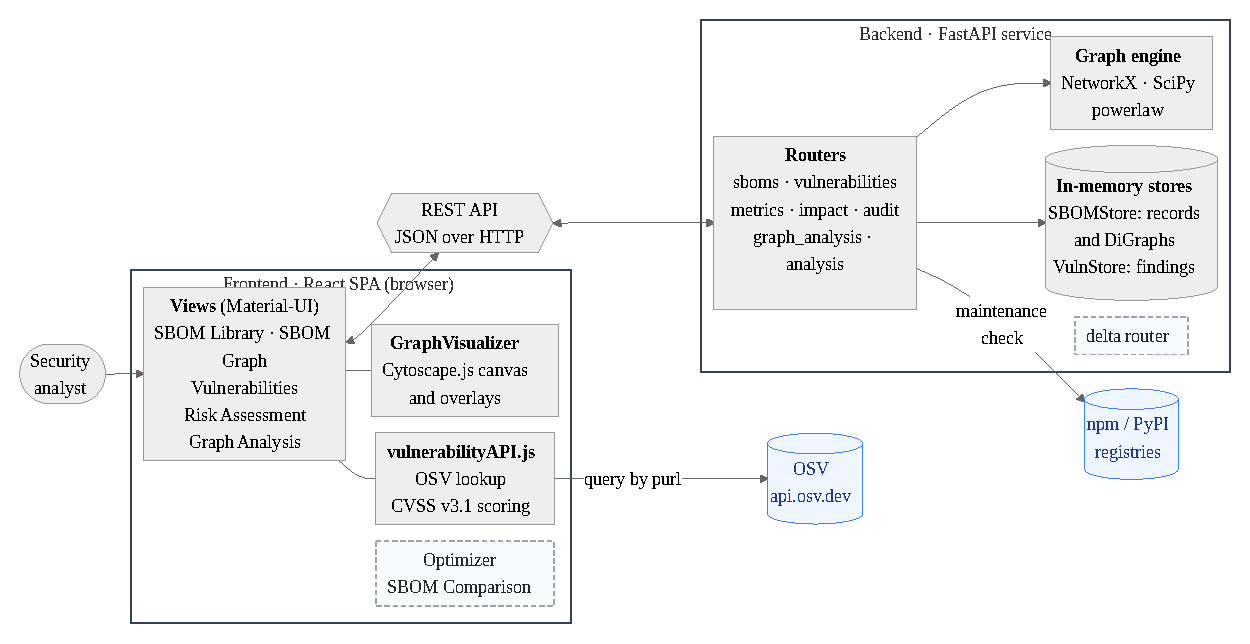
\includegraphics[width=\textwidth]{Figures/Chapter4/architecture.pdf}
%     \caption[SBOM Lens system architecture]{SBOM Lens three-layer architecture. Modules outside the thesis scope (Topology Optimiser, Comparison/Delta) are visually distinguished.}
%     \label{fig:architecture}
% \end{figure}


\subsection{Frontend Layer}
\label{sec:frontend}

The frontend is a React single-page application styled with the Material-UI (MUI) component library. It exposes three primary views: the SBOM Graph (the central visualisation canvas), the Vulnerability Dashboard (aggregated CVE data and remediation status), and the Graph Analysis panel (network-science metric display). A persistent side navigation bar connects the views and hosts the SBOM selection control.

Graph rendering is delegated entirely to Cytoscape.js through a \texttt{GraphVisualizer} React component that holds the Cytoscape instance in a \texttt{useRef} hook. This architectural choice is deliberate: Cytoscape.js manages the HTML5 canvas directly and responds to user gestures with sub-millisecond latency. Routing all canvas operations through React's virtual-DOM reconciler would introduce unnecessary re-render overhead for every pan, zoom, or node drag event. React manages application state --- which SBOM is loaded, which analysis mode is active --- while Cytoscape manages the visual representation.

The data layer is controlled by a compile-time constant \texttt{DATA\_SOURCE} defined in the application configuration file. It switches between \texttt{'localStorage'} (an offline convenience mode used during frontend development) and \texttt{'api'} (the production path that calls the FastAPI backend). The thesis evaluation uses the \texttt{'api'} mode exclusively. The analysis toolbar, which exposes the overlay modes described in \autoref{cp:vuln-analysis} and \autoref{cp:network-sci}, is visible only in API mode when an SBOM is loaded.


\subsection{Backend Layer}
\label{sec:backend}

The backend is a FastAPI application defined in \texttt{main.py} with seven routers registered at startup: \texttt{sboms}, \texttt{vulnerabilities}, \texttt{metrics}, \texttt{impact}, \texttt{audit}, \texttt{graph\_analysis}, and \texttt{delta}. Registration order is significant: the \texttt{delta} and \texttt{graph\_analysis} routers are registered before \texttt{sboms} to prevent FastAPI's wildcard path parameter \texttt{\{sbom\_id\}} from greedily intercepting fixed paths such as \texttt{/sboms/compare}.

The graph engine is NetworkX's \texttt{DiGraph} class. All structural algorithms operate directly on the stored \texttt{DiGraph} object: these include articulation-point detection, k-core decomposition, HITS centrality, Louvain community detection, spectral radius estimation, and the epidemic propagation model, all described in \autoref{cp:network-sci}. This avoids any serialisation step between storage and computation: the router receives a Python object reference, runs the algorithm, and returns results without intermediate conversion.

Several routers maintain per-SBOM result caches at the module level. Community detection and k-core results are expensive to recompute for large graphs; caching ensures that repeated requests for the same SBOM complete in constant time. All caches are explicitly invalidated when an SBOM is updated or deleted, guaranteeing consistency between the stored graph and any cached analytical results.


\subsection{Communication: REST API}
\label{sec:rest-api}

The REST API is served at \texttt{http://localhost:8000} by default, overridable via an environment variable. CORS is configured to permit requests from the React development server. A health endpoint at \texttt{GET /health} returns a JSON object confirming the service status and version number; the frontend uses this to detect backend availability before enabling API-mode features.

The endpoints directly relevant to this chapter are: \texttt{POST /sboms} (file upload, graph construction, and storage), \texttt{GET /sboms/\{id\}} (retrieve a stored SBOM record), and \texttt{GET /sboms/\{id\}/metrics} (returns graph-level metrics including node count, edge count, average out-degree, and the five most-depended-on components ranked by in-degree). The remaining endpoints --- \texttt{/vulnerabilities}, \texttt{/\{id\}/impact}, \texttt{/\{id\}/audit}, \texttt{/\{id\}/graph-analysis}, \texttt{/\{id\}/kcore}, \texttt{/\{id\}/communities}, and \texttt{/\{id\}/epidemic} --- are described in \autoref{cp:vuln-analysis} and \autoref{cp:network-sci} respectively.


\section{CycloneDX Parsing Pipeline}
\label{sec:parsing-pipeline}

Every SBOM in SBOM Lens enters through a single ingest endpoint and exits as a cached \texttt{nx.DiGraph} that all downstream routers query directly. The pipeline is designed for a ``parse once, query many times'' pattern: the graph is built on first ingest and never re-parsed unless the SBOM is explicitly updated. The three subsections trace each stage: upload and duplicate detection, component extraction and node creation, and dependency iteration and edge construction.


\subsection{Ingestion and Deduplication}
\label{sec:ingestion}

SBOM ingestion begins at the \texttt{POST /sboms} endpoint, which accepts a multipart file upload. The raw file bytes are read in full before any graph construction begins, allowing the system to perform two correctness checks upfront.

The first check is JSON validation. The raw bytes are passed to \texttt{json.loads()}; if parsing fails, an HTTP 400 response is returned immediately. This guard ensures that no partially constructed graph can enter the store from a malformed file.

The second check is duplicate detection. A SHA-256 hash of the raw file bytes is computed with \texttt{hashlib.sha256(contents).hexdigest()} and compared against the \texttt{"hash"} field of every stored SBOM record. If a match is found, the endpoint returns \texttt{\{"isDuplicate": True, "existingSBOM": existing\}} without re-storing the file or reconstructing the graph. This ``parse once, query many times'' design avoids redundant computation and prevents double-counting in metrics when the same SBOM is submitted more than once.

A capacity limit prevents unbounded memory growth: the \texttt{MAX\_SBOMS} environment variable (default: 10) caps the number of concurrently stored SBOMs. An upload that would exceed the limit is rejected with HTTP 409 Conflict. This limit is appropriate for a research prototype evaluated on a fixed dataset.


\subsection{Component Extraction}
\label{sec:component-extraction}

Once the file passes validation and deduplication, the CycloneDX JSON structure is traversed to extract components. The root component --- the project or application being described by the SBOM --- is extracted from the \texttt{metadata.component} field and prepended to the \texttt{components[]} list. This placement gives the root a consistent position in the graph and allows the frontend to distinguish it visually as the primary node.

Each entry in the assembled component list is processed into a NetworkX node. The node identifier is resolved through a three-level fallback chain: \texttt{bom-ref} (the CycloneDX primary identifier) is used if present; otherwise \texttt{purl} (Package URL) is used; otherwise the component \texttt{name}. This chain mirrors the CycloneDX field hierarchy defined in \autoref{sec:sbom-cyclonedx} and ensures stable, unique node identifiers across SBOMs produced by different tools with varying levels of metadata completeness.

Node attributes are stored as the NetworkX node's data dictionary. To avoid compatibility issues with NetworkX's attribute handling, only scalar values --- strings, integers, floats, and booleans --- are retained from the component object. In practice, the persisted attributes are \texttt{name}, \texttt{version}, \texttt{purl}, \texttt{type}, and \texttt{bom-ref}. Components for which all three identifier fallbacks yield an empty or \texttt{None} value are silently skipped, making the parser tolerant of incomplete SBOMs encountered in the wild.


\subsection{Graph Construction from Dependencies}
\label{sec:graph-construction}

After all nodes are created, the \texttt{dependencies[]} array is iterated to construct directed edges. Each entry in this array follows the CycloneDX dependency schema: a \texttt{ref} field identifying the depending component, and a \texttt{dependsOn} list identifying the components it depends upon. For each \texttt{(ref, target)} pair, a directed edge is added to the graph with \texttt{G.add\_edge(ref, target)}.

The edge direction encodes a fundamental semantic: an edge from A to B means ``A depends on B''. This directed convention underpins all downstream traversal algorithms. Blast-radius computation, for example, uses \texttt{nx.ancestors(G, node\_id)} to find all components that transitively depend on a given node --- ancestors in the directed graph are precisely those dependants, consistent with the \texttt{ref} \(\to\) \texttt{target} edge direction.

Before adding each edge, a guard verifies that both \texttt{ref} and \texttt{target} already exist as nodes in the graph. Entries in \texttt{dependencies[]} that reference undeclared components are silently skipped. This tolerance is necessary because real-world SBOMs do not always maintain a complete correspondence between the \texttt{components[]} and \texttt{dependencies[]} sections.

The resulting \texttt{nx.DiGraph} is stored in \texttt{SBOMStore.graphs[sbom\_id]} and never re-parsed unless the SBOM is explicitly updated via \texttt{PUT /sboms/\{id\}}. All downstream routers retrieve the graph by calling \texttt{sbom\_store.get\_graph(sbom\_id)}, receiving a direct reference to the live \texttt{DiGraph} object with zero serialisation overhead.


\section{Graph Data Model}
\label{sec:graph-data-model}

The directed graph constructed by the parsing pipeline (\autoref{sec:parsing-pipeline}) encodes the SBOM's component and dependency structure in a form that all downstream algorithms can consume directly. This section defines the node and edge data model --- the representation used by all algorithms in \autoref{cp:vuln-analysis} and \autoref{cp:network-sci}. The in-memory store that manages graph lifecycle is described last.


\subsection{Node Representation}
\label{sec:node-representation}

Each node in the \texttt{DiGraph} represents one software component as declared in the CycloneDX SBOM. The graph contains exactly one node per distinct component identifier, as determined by the \texttt{bom-ref}/\texttt{purl}/\texttt{name} fallback chain described in \autoref{sec:component-extraction}. The node identifier --- the key used to reference the node in all NetworkX operations --- is a stable string assigned at ingest time and unchanged for the lifetime of the stored SBOM.

Each node carries a data dictionary with the following attributes:

\begin{itemize}
    \item \texttt{name} --- human-readable display label for the component.
    \item \texttt{version} --- semantic version string as declared in the SBOM.
    \item \texttt{purl} --- Package URL, used as the primary lookup key when matching components against vulnerability databases in \autoref{cp:vuln-analysis}.
    \item \texttt{type} --- CycloneDX component type; one of \texttt{library}, \texttt{framework}, or \texttt{application}.
    \item \texttt{bom-ref} --- the original CycloneDX \texttt{bom-ref} string, preserved for traceability back to the source file.
\end{itemize}

The root component (extracted from \texttt{metadata.component}) is a regular node in the NetworkX graph. The frontend distinguishes it visually by setting an \texttt{isPrimary} flag in the Cytoscape node data object produced by \texttt{convertCycloneDXToGraph()}, which triggers a distinct green fill on the canvas.


\subsection{Edge Representation}
\label{sec:edge-representation}

Each directed edge represents a direct dependency relationship between two components. An edge from node A to node B encodes the statement: \textit{A directly depends on B}. This follows from the CycloneDX dependency schema, where an entry \texttt{(ref: A, dependsOn: [B, ...])} produces the directed edge A \(\to\) B.

This directed semantics is load-bearing for every traversal algorithm in the system. Blast-radius analysis identifies all components that would be affected if a given component were compromised; these are its \textit{ancestors} in the directed graph --- the nodes from which there exists a directed path to the target, consistent with the A \(\to\) B convention. Dominator-tree construction, depth histograms, and topological ordering all depend on the same directed convention, as described in \autoref{cp:vuln-analysis} and \autoref{cp:network-sci}.

No attributes are stored on NetworkX edges. Edges are pure structural connectors: their presence encodes a dependency, and their direction encodes which component depends on which. On the frontend, each Cytoscape edge object carries an identifier formed from the source and target node IDs, a static label \texttt{depends\_on}, and the CSS class \texttt{default-edge} for baseline styling.


\subsection{In-Memory Store}
\label{sec:in-memory-store}

The \texttt{SBOMStore} class manages the lifecycle of all stored SBOMs and their corresponding graphs. It maintains two parallel dictionaries: \texttt{self.sboms} maps each SBOM identifier to a full record dictionary (containing the SHA-256 hash, display name, creation timestamp, and the raw CycloneDX component and dependency lists); \texttt{self.graphs} maps the same identifier to the corresponding \texttt{nx.DiGraph}.

When a router needs to perform graph analysis, it retrieves the stored \texttt{DiGraph} via the store's \texttt{get\_graph} method, which returns a direct Python reference to the live object. There is no serialisation step between storage and computation: the algorithm receives the graph object and operates on it in place. This design minimises latency for interactive analysis queries, where sub-second response times are necessary for a usable graph exploration interface.

Several routers maintain module-level caches for computationally expensive results --- community detection and k-core decomposition are cached after the first request for a given SBOM. These caches are explicitly invalidated whenever an SBOM is updated or deleted, ensuring that stale results are never returned to the frontend.

As noted in \autoref{sec:architecture-overview}, the store's state is ephemeral: a server restart clears all SBOMs and graphs. This design is appropriate for the research context, and persistent storage is listed as a limitation and direction for future work in \autoref{cp:conclusion}.


\section{SBOM Graph Visualisation}
\label{sec:graph-visualisation}

The SBOM Graph is the primary interface through which the user explores the dependency structure of a loaded SBOM. This section describes the base rendering layer implemented with Cytoscape.js, the three available layout algorithms, and the core interaction model. Analysis overlays --- vulnerability highlighting (\autoref{cp:vuln-analysis}) and network-science colouring (\autoref{cp:network-sci}) --- extend the base layer described here.


\subsection{Graph Rendering with Cytoscape.js}
\label{sec:cytoscape-rendering}

Cytoscape.js is initialised imperatively inside the \texttt{GraphVisualizer} React component using the \texttt{useRef} and \texttt{useEffect} hooks. The Cytoscape instance is stored in a ref rather than component state, so operations on the canvas --- panning, zooming, applying a new layout --- do not trigger React's reconciliation cycle. This separation keeps the graph canvas responsive under interactive load.

The default visual encoding uses a consistent style throughout the application. Component nodes are rendered as circular shapes (\(28 \times 28\) pixels) filled with Material-UI's info blue, with the component name displayed as a label below the node. The root component --- the project whose dependencies are being analysed --- is distinguished by a green fill and a 2-pixel border, making it immediately identifiable as the anchor of the dependency tree. Dependency edges are rendered as Bézier curves with triangle arrowheads at the target end, indicating the direction of dependency. Edges carry the static label \texttt{depends\_on} with auto-rotate enabled so the label follows the curve.

Overlay CSS classes are pre-defined in the Cytoscape stylesheet and applied programmatically when an analysis mode is activated. The pre-defined overlay classes are: \texttt{.articulation-point} (red), \texttt{.blast-radius} (purple), \texttt{.dominator-tree} (cyan), \texttt{.vuln-node} (orange), \texttt{.diamond-node} (green), and \texttt{.hits-active} (node size and colour scaled from HITS score attributes). A \texttt{.dimmed} class reduces opacity to 15\,\% to grey out nodes and edges that are not part of the current selection or overlay. The analytical meaning of each overlay class is defined in \autoref{cp:vuln-analysis} and \autoref{cp:network-sci}; this section establishes the visual layer only.


\subsection{Layout Algorithms}
\label{sec:layouts}

SBOM Lens exposes three Cytoscape.js layout algorithms, accessible via toolbar buttons, each suited to a different graph exploration objective.

The \textbf{Tree Layout} (Cytoscape name: \texttt{breadthfirst}, \texttt{directed: true}) organises nodes in horizontal levels according to their distance from the root in a breadth-first traversal. This layout makes dependency depth immediately visible: direct dependencies appear on level one, transitive dependencies on level two and beyond. It is the default layout for the Delta and Comparison views, where structural differences between two SBOMs are easier to compare when both graphs share the same hierarchical orientation.

The \textbf{Radial Layout} (Cytoscape name: \texttt{concentric}) places nodes in concentric rings around a central hub, with the root component at the centre. This is the default layout applied when a new SBOM is first loaded, giving the user an immediate overview of the dependency neighbourhood around the root.

The \textbf{Force-Directed Layout} (Cytoscape name: \texttt{cose}) simulates a physical spring system to distribute nodes so that connected components cluster together organically without imposing a hierarchical structure. This layout is particularly effective for revealing natural groupings in large, densely connected SBOMs.

All three layouts share common configuration options: \texttt{fit: true} (zoom to fit the graph on screen), a padding of 150 pixels, overlap avoidance, and an animated transition of 600\,ms. Layout changes are applied imperatively by re-running the Cytoscape algorithm on the existing node and edge data without issuing a new request to the backend.


\subsection{Core Interaction Model}
\label{sec:interaction-model}

The SBOM Graph supports the following core interactions, designed to enable focused exploration of the dependency structure.

\textbf{Node selection.} Tapping a node selects it; a blue border is applied to the highlighted node. Tapping the canvas background deselects all nodes.

\textbf{Node inspection.} Selecting a node opens a sidebar panel displaying the node's stored attributes: \texttt{name}, \texttt{version}, \texttt{purl}, \texttt{type}, and \texttt{bom-ref}. This panel gives the analyst the metadata needed to cross-reference the selected component with external vulnerability databases.

\textbf{Zoom and fit.} The current zoom level is tracked in React component state and displayed in the toolbar. A fit-to-view button resets the viewport so the entire graph is visible, which is useful after navigating to a deeply nested subgraph.

\textbf{SBOM selection.} A selector component lists all SBOMs currently stored in \texttt{SBOMStore}. Selecting an SBOM converts the stored CycloneDX data to Cytoscape node and edge objects and loads them into the Cytoscape instance.

\textbf{Impact analysis entry point.} Right-clicking a node opens a context menu that includes an impact analysis option, which fetches blast-radius and dominator-tree data from the backend. The analytical meaning of the resulting overlay is described in \autoref{cp:vuln-analysis}; the interaction gesture is documented here as part of the interaction model.

Dynamic graph editing features --- adding new nodes, repositioning nodes by dragging, and creating edges via the \texttt{cytoscape-edgehandles} plugin --- are implemented in the application but are outside the scope of this thesis. These are graph construction utilities, not structural risk assessment features, and are not evaluated in this work.
